\documentclass{standalone}
\usepackage{tikz}
\usetikzlibrary{patterns, positioning}

\begin{document}
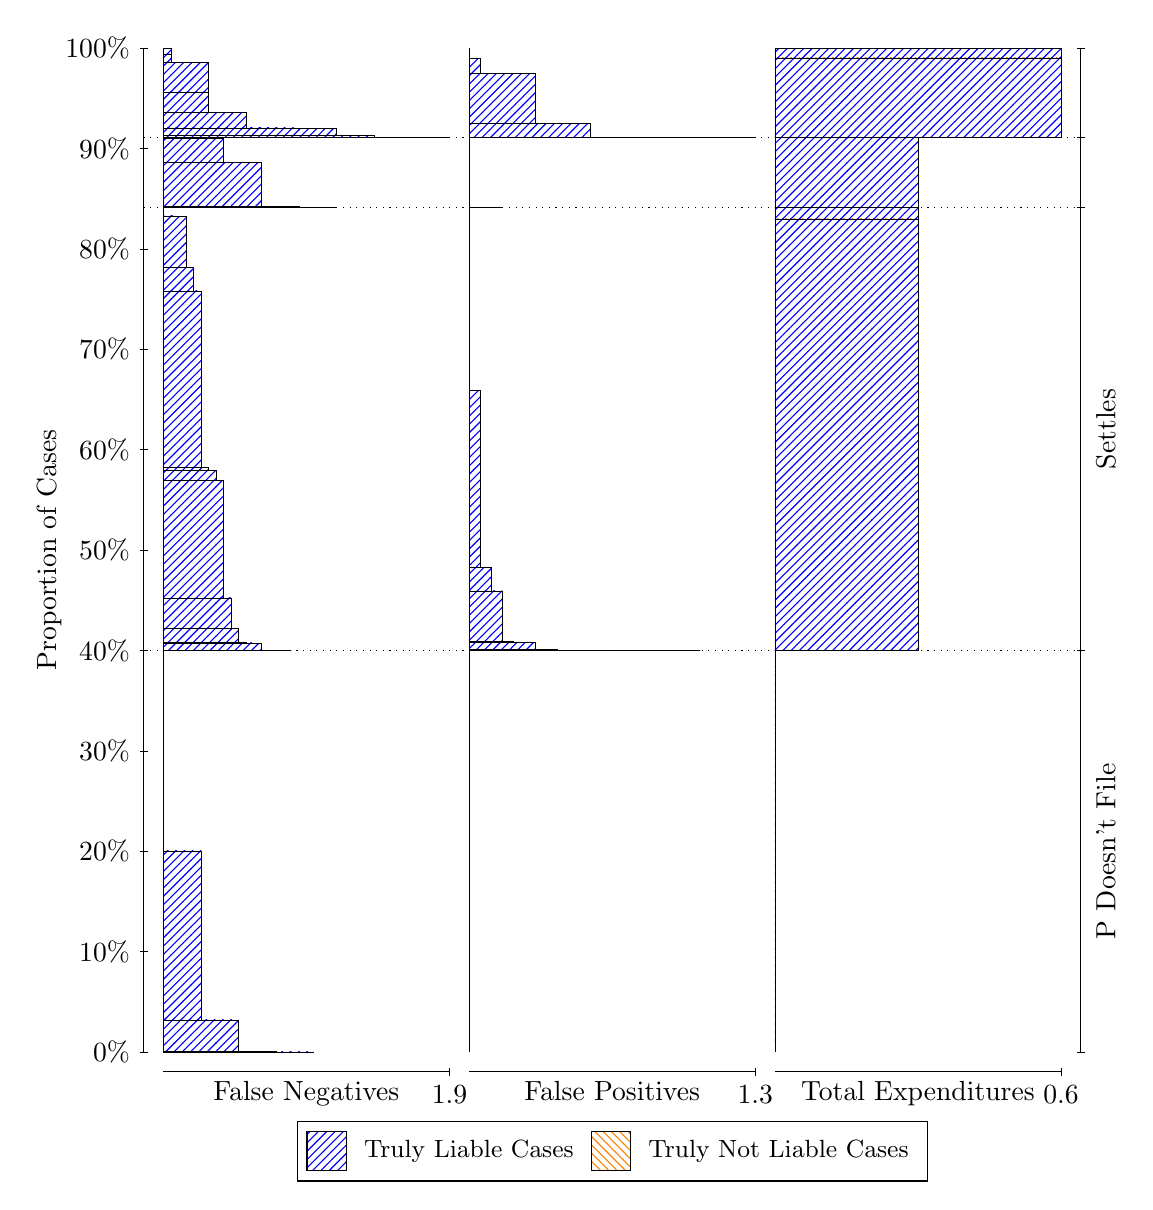
\begin{tikzpicture}
\draw[black, very thin] (1.5,1.75) -- (1.5,14.5);
\node[rotate=90, anchor=center] at (0.3, 8.125) {Proportion of Cases};
\draw[black, very thin] (1.45,1.75) -- (1.55,1.75);
\node[anchor=east] at (1.45, 1.75) {0\%};
\draw[black, very thin] (1.45,3.025) -- (1.55,3.025);
\node[anchor=east] at (1.45, 3.025) {10\%};
\draw[black, very thin] (1.45,4.3) -- (1.55,4.3);
\node[anchor=east] at (1.45, 4.3) {20\%};
\draw[black, very thin] (1.45,5.575) -- (1.55,5.575);
\node[anchor=east] at (1.45, 5.575) {30\%};
\draw[black, very thin] (1.45,6.85) -- (1.55,6.85);
\node[anchor=east] at (1.45, 6.85) {40\%};
\draw[black, very thin] (1.45,8.125) -- (1.55,8.125);
\node[anchor=east] at (1.45, 8.125) {50\%};
\draw[black, very thin] (1.45,9.4) -- (1.55,9.4);
\node[anchor=east] at (1.45, 9.4) {60\%};
\draw[black, very thin] (1.45,10.675) -- (1.55,10.675);
\node[anchor=east] at (1.45, 10.675) {70\%};
\draw[black, very thin] (1.45,11.95) -- (1.55,11.95);
\node[anchor=east] at (1.45, 11.95) {80\%};
\draw[black, very thin] (1.45,13.225) -- (1.55,13.225);
\node[anchor=east] at (1.45, 13.225) {90\%};
\draw[black, very thin] (1.45,14.5) -- (1.55,14.5);
\node[anchor=east] at (1.45, 14.5) {100\%};

\draw[black, very thin] (13.4,1.75) -- (13.4,14.5);
\draw[black, very thin] (13.35,1.75) -- (13.45,1.75);
\node[anchor=west] at (13.35, 1.75) {};
\draw[black, very thin] (13.35,6.8489) -- (13.45,6.8489);
\node[anchor=west] at (13.35, 6.8489) {};
\draw[black, very thin] (13.35,12.473) -- (13.45,12.473);
\node[anchor=west] at (13.35, 12.473) {};
\draw[black, very thin] (13.35,13.361) -- (13.45,13.361);
\node[anchor=west] at (13.35, 13.361) {};
\draw[black, very thin] (13.35,14.5) -- (13.45,14.5);
\node[anchor=west] at (13.35, 14.5) {};

\draw[black, very thin, pattern color=blue, pattern=north east lines] (1.75,1.75) rectangle (3.6623,1.75);
\draw[black, very thin, pattern color=blue, pattern=north east lines] (1.75,1.75) rectangle (3.1842,1.7534);
\draw[black, very thin, pattern color=blue, pattern=north east lines] (1.75,1.7534) rectangle (2.7061,2.158);
\draw[black, very thin, pattern color=blue, pattern=north east lines] (1.75,2.158) rectangle (2.2281,4.3029);
\draw[black, very thin, pattern color=orange, pattern=north west lines] (1.75,4.3029) rectangle (1.75,4.3029);
\draw[black, very thin, pattern color=blue, pattern=north east lines] (1.75,4.3029) rectangle (1.75,6.8489);
\draw[black, very thin, pattern color=blue, pattern=north east lines] (1.75,6.8489) rectangle (3.3754,6.8489);
\draw[black, very thin, pattern color=blue, pattern=north east lines] (1.75,6.8489) rectangle (3.1842,6.8493);
\draw[black, very thin, pattern color=blue, pattern=north east lines] (1.75,6.8493) rectangle (2.993,6.9392);
\draw[black, very thin, pattern color=blue, pattern=north east lines] (1.75,6.9392) rectangle (2.8974,6.9461);
\draw[black, very thin, pattern color=blue, pattern=north east lines] (1.75,6.9461) rectangle (2.8018,6.948);
\draw[black, very thin, pattern color=blue, pattern=north east lines] (1.75,6.948) rectangle (2.7061,7.1277);
\draw[black, very thin, pattern color=blue, pattern=north east lines] (1.75,7.1277) rectangle (2.6105,7.5159);
\draw[black, very thin, pattern color=blue, pattern=north east lines] (1.75,7.5159) rectangle (2.5149,9.0043);
\draw[black, very thin, pattern color=blue, pattern=north east lines] (1.75,9.0043) rectangle (2.4193,9.1339);
\draw[black, very thin, pattern color=blue, pattern=north east lines] (1.75,9.1339) rectangle (2.3237,9.1703);
\draw[black, very thin, pattern color=blue, pattern=north east lines] (1.75,9.1703) rectangle (2.2281,11.415);
\draw[black, very thin, pattern color=blue, pattern=north east lines] (1.75,11.415) rectangle (2.1325,11.716);
\draw[black, very thin, pattern color=blue, pattern=north east lines] (1.75,11.716) rectangle (2.0368,12.361);
\draw[black, very thin, pattern color=blue, pattern=north east lines] (1.75,12.361) rectangle (1.9412,12.368);
\draw[black, very thin, pattern color=blue, pattern=north east lines] (1.75,12.368) rectangle (1.8456,12.369);
\draw[black, very thin, pattern color=orange, pattern=north west lines] (1.75,12.369) rectangle (1.75,12.369);
\draw[black, very thin, pattern color=blue, pattern=north east lines] (1.75,12.369) rectangle (1.75,12.473);
\draw[black, very thin, pattern color=blue, pattern=north east lines] (1.75,12.473) rectangle (3.9491,12.473);
\draw[black, very thin, pattern color=blue, pattern=north east lines] (1.75,12.473) rectangle (3.4711,12.49);
\draw[black, very thin, pattern color=blue, pattern=north east lines] (1.75,12.49) rectangle (2.993,13.046);
\draw[black, very thin, pattern color=blue, pattern=north east lines] (1.75,13.046) rectangle (2.5149,13.357);
\draw[black, very thin, pattern color=blue, pattern=north east lines] (1.75,13.357) rectangle (2.0368,13.361);
\draw[black, very thin, pattern color=orange, pattern=north west lines] (1.75,13.361) rectangle (1.75,13.361);
\draw[black, very thin, pattern color=blue, pattern=north east lines] (1.75,13.361) rectangle (5.3833,13.361);
\draw[black, very thin, pattern color=blue, pattern=north east lines] (1.75,13.361) rectangle (4.9053,13.361);
\draw[black, very thin, pattern color=blue, pattern=north east lines] (1.75,13.361) rectangle (4.4272,13.387);
\draw[black, very thin, pattern color=blue, pattern=north east lines] (1.75,13.387) rectangle (3.9491,13.484);
\draw[black, very thin, pattern color=blue, pattern=north east lines] (1.75,13.484) rectangle (3.7579,13.484);
\draw[black, very thin, pattern color=blue, pattern=north east lines] (1.75,13.484) rectangle (3.4711,13.486);
\draw[black, very thin, pattern color=blue, pattern=north east lines] (1.75,13.486) rectangle (3.2798,13.487);
\draw[black, very thin, pattern color=blue, pattern=north east lines] (1.75,13.487) rectangle (2.993,13.487);
\draw[black, very thin, pattern color=blue, pattern=north east lines] (1.75,13.487) rectangle (2.8018,13.685);
\draw[black, very thin, pattern color=blue, pattern=north east lines] (1.75,13.685) rectangle (2.5149,13.685);
\draw[black, very thin, pattern color=blue, pattern=north east lines] (1.75,13.685) rectangle (2.3237,13.943);
\draw[black, very thin, pattern color=blue, pattern=north east lines] (1.75,13.943) rectangle (2.3237,14.319);
\draw[black, very thin, pattern color=blue, pattern=north east lines] (1.75,14.319) rectangle (1.8456,14.425);
\draw[black, very thin, pattern color=blue, pattern=north east lines] (1.75,14.425) rectangle (1.8456,14.493);
\draw[black, very thin, pattern color=orange, pattern=north west lines] (1.75,14.493) rectangle (1.75,14.493);
\draw[black, very thin, pattern color=blue, pattern=north east lines] (1.75,14.493) rectangle (1.75,14.5);
\draw[black, very thin, pattern color=orange, pattern=north west lines] (5.6333,1.75) rectangle (5.6333,1.75);
\draw[black, very thin, pattern color=blue, pattern=north east lines] (5.6333,1.75) rectangle (5.6333,6.8489);
\draw[black, very thin, pattern color=orange, pattern=north west lines] (5.6333,6.8489) rectangle (8.5679,6.8489);
\draw[black, very thin, pattern color=blue, pattern=north east lines] (5.6333,6.8489) rectangle (8.5679,6.8489);
\draw[black, very thin, pattern color=orange, pattern=north west lines] (5.6333,6.8489) rectangle (8.009,6.8489);
\draw[black, very thin, pattern color=blue, pattern=north east lines] (5.6333,6.8489) rectangle (8.009,6.8489);
\draw[black, very thin, pattern color=blue, pattern=north east lines] (5.6333,6.8489) rectangle (7.8692,6.8489);
\draw[black, very thin, pattern color=orange, pattern=north west lines] (5.6333,6.8489) rectangle (7.7295,6.8489);
\draw[black, very thin, pattern color=blue, pattern=north east lines] (5.6333,6.8489) rectangle (7.7295,6.8489);
\draw[black, very thin, pattern color=orange, pattern=north west lines] (5.6333,6.8489) rectangle (7.45,6.8489);
\draw[black, very thin, pattern color=blue, pattern=north east lines] (5.6333,6.8489) rectangle (7.45,6.8489);
\draw[black, very thin, pattern color=blue, pattern=north east lines] (5.6333,6.8489) rectangle (7.3103,6.8489);
\draw[black, very thin, pattern color=orange, pattern=north west lines] (5.6333,6.8489) rectangle (7.1705,6.8489);
\draw[black, very thin, pattern color=blue, pattern=north east lines] (5.6333,6.8489) rectangle (7.1705,6.8489);
\draw[black, very thin, pattern color=blue, pattern=north east lines] (5.6333,6.8489) rectangle (7.0308,6.8489);
\draw[black, very thin, pattern color=orange, pattern=north west lines] (5.6333,6.8489) rectangle (6.891,6.8489);
\draw[black, very thin, pattern color=blue, pattern=north east lines] (5.6333,6.8489) rectangle (6.891,6.8489);
\draw[black, very thin, pattern color=blue, pattern=north east lines] (5.6333,6.8489) rectangle (6.7513,6.8655);
\draw[black, very thin, pattern color=blue, pattern=north east lines] (5.6333,6.8655) rectangle (6.6115,6.867);
\draw[black, very thin, pattern color=blue, pattern=north east lines] (5.6333,6.867) rectangle (6.4718,6.9523);
\draw[black, very thin, pattern color=blue, pattern=north east lines] (5.6333,6.9523) rectangle (6.3321,6.9537);
\draw[black, very thin, pattern color=blue, pattern=north east lines] (5.6333,6.9537) rectangle (6.1923,6.9606);
\draw[black, very thin, pattern color=blue, pattern=north east lines] (5.6333,6.9606) rectangle (6.0526,7.6051);
\draw[black, very thin, pattern color=blue, pattern=north east lines] (5.6333,7.6051) rectangle (5.9128,7.9066);
\draw[black, very thin, pattern color=blue, pattern=north east lines] (5.6333,7.9066) rectangle (5.7731,10.151);
\draw[black, very thin, pattern color=blue, pattern=north east lines] (5.6333,10.151) rectangle (5.6333,12.473);
\draw[black, very thin, pattern color=orange, pattern=north west lines] (5.6333,12.473) rectangle (6.0526,12.473);
\draw[black, very thin, pattern color=blue, pattern=north east lines] (5.6333,12.473) rectangle (6.0526,12.476);
\draw[black, very thin, pattern color=blue, pattern=north east lines] (5.6333,12.476) rectangle (5.6333,13.361);
\draw[black, very thin, pattern color=orange, pattern=north west lines] (5.6333,13.361) rectangle (9.2667,13.361);
\draw[black, very thin, pattern color=blue, pattern=north east lines] (5.6333,13.361) rectangle (9.2667,13.361);
\draw[black, very thin, pattern color=orange, pattern=north west lines] (5.6333,13.361) rectangle (8.5679,13.361);
\draw[black, very thin, pattern color=blue, pattern=north east lines] (5.6333,13.361) rectangle (8.5679,13.361);
\draw[black, very thin, pattern color=orange, pattern=north west lines] (5.6333,13.361) rectangle (7.8692,13.361);
\draw[black, very thin, pattern color=blue, pattern=north east lines] (5.6333,13.361) rectangle (7.8692,13.367);
\draw[black, very thin, pattern color=orange, pattern=north west lines] (5.6333,13.367) rectangle (7.1705,13.367);
\draw[black, very thin, pattern color=blue, pattern=north east lines] (5.6333,13.367) rectangle (7.1705,13.542);
\draw[black, very thin, pattern color=blue, pattern=north east lines] (5.6333,13.542) rectangle (6.4718,14.176);
\draw[black, very thin, pattern color=orange, pattern=north west lines] (5.6333,14.176) rectangle (6.1923,14.176);
\draw[black, very thin, pattern color=blue, pattern=north east lines] (5.6333,14.176) rectangle (6.1923,14.176);
\draw[black, very thin, pattern color=blue, pattern=north east lines] (5.6333,14.176) rectangle (5.7731,14.373);
\draw[black, very thin, pattern color=orange, pattern=north west lines] (5.6333,14.373) rectangle (5.6333,14.373);
\draw[black, very thin, pattern color=blue, pattern=north east lines] (5.6333,14.373) rectangle (5.6333,14.5);
\draw[black, very thin, pattern color=orange, pattern=north west lines] (9.5167,1.75) rectangle (9.5167,1.75);
\draw[black, very thin, pattern color=blue, pattern=north east lines] (9.5167,1.75) rectangle (9.5167,6.8489);
\draw[black, very thin, pattern color=orange, pattern=north west lines] (9.5167,6.8489) rectangle (11.333,6.8489);
\draw[black, very thin, pattern color=blue, pattern=north east lines] (9.5167,6.8489) rectangle (11.333,12.329);
\draw[black, very thin, pattern color=orange, pattern=north west lines] (9.5167,12.329) rectangle (11.333,12.329);
\draw[black, very thin, pattern color=blue, pattern=north east lines] (9.5167,12.329) rectangle (11.333,12.473);
\draw[black, very thin, pattern color=orange, pattern=north west lines] (9.5167,12.473) rectangle (11.333,12.473);
\draw[black, very thin, pattern color=blue, pattern=north east lines] (9.5167,12.473) rectangle (11.333,13.361);
\draw[black, very thin, pattern color=orange, pattern=north west lines] (9.5167,13.361) rectangle (13.15,13.361);
\draw[black, very thin, pattern color=blue, pattern=north east lines] (9.5167,13.361) rectangle (13.15,14.375);
\draw[black, very thin, pattern color=orange, pattern=north west lines] (9.5167,14.375) rectangle (13.15,14.375);
\draw[black, very thin, pattern color=blue, pattern=north east lines] (9.5167,14.375) rectangle (13.15,14.5);
\draw[black, dotted] (1.5,6.8489) -- (13.4,6.8489);
\draw[black, dotted] (1.5,12.473) -- (13.4,12.473);
\draw[black, dotted] (1.5,13.361) -- (13.4,13.361);
\draw[black, very thin] (1.75,1.5) -- (5.3833,1.5);
\node[anchor=north] at (3.5667, 1.5) {False Negatives};
\draw[black, very thin] (5.3833,1.45) -- (5.3833,1.55);
\node[anchor=north] at (5.3833, 1.45) {1.9};

\draw[black, very thin] (5.6333,1.5) -- (9.2667,1.5);
\node[anchor=north] at (7.45, 1.5) {False Positives};
\draw[black, very thin] (9.2667,1.45) -- (9.2667,1.55);
\node[anchor=north] at (9.2667, 1.45) {1.3};

\draw[black, very thin] (9.5167,1.5) -- (13.15,1.5);
\node[anchor=north] at (11.333, 1.5) {Total Expenditures};
\draw[black, very thin] (13.15,1.45) -- (13.15,1.55);
\node[anchor=north] at (13.15, 1.45) {0.6};

\node[black, centered, rotate=90] at (13.72, 4.2994) {P Doesn't File};
\node[black, centered, rotate=90] at (13.72, 9.6607) {Settles};



\draw (7.449999999999999,1.5) node[draw=none] (baseCoordinate) {};
\begin{scope}[align=center]
        \matrix[scale=0.5, draw=black, below=0.5cm of baseCoordinate, nodes={draw}, column sep=0.1cm]{
            \node[rectangle, draw, minimum width=0.5cm, minimum height=0.5cm, pattern=north east lines, pattern color=blue] {}; &
            \node[draw=none, font=\small] (B) {Truly Liable Cases}; &
            \node[rectangle, draw, minimum width=0.5cm, minimum height=0.5cm, pattern=north west lines, pattern color=orange] {}; &
            \node[draw=none, font=\small] (B) {Truly Not Liable Cases}; \\
            };
\end{scope}

\end{tikzpicture}
\end{document}